
\documentclass[tikz,border=10pt]{standalone}
\begin{document}

    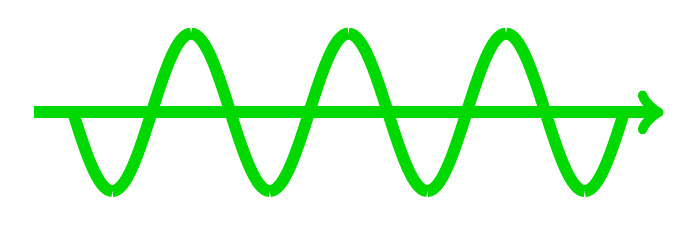
\begin{tikzpicture}

    \draw[ultra thick,color=black!15!green,line width=1.5mm,->] (4,0) -- (12,0);
    % \draw[ultra thick, color=black!15!green,line width=1.5mm] (4,1) cos (4.5,0);
    \draw[ultra thick, color=black!15!green,line width=1.5mm] (4.5,0) sin (5,-1);
    \draw[ultra thick, color=black!15!green,line width=1.5mm] (5,-1) cos (5.5,0);
    \draw[ultra thick, color=black!15!green,line width=1.5mm] (5.5,0)  sin (6,1);
    \draw[ultra thick, color=black!15!green,line width=1.5mm] (6,1) cos (6.5,0);
    \draw[ultra thick, color=black!15!green,line width=1.5mm] (6.5,0) sin (7,-1);
    \draw[ultra thick, color=black!15!green,line width=1.5mm] (7,-1) cos (7.5,0);
    \draw[ultra thick, color=black!15!green,line width=1.5mm] (7.5,0) sin (8,1);
    \draw[ultra thick, color=black!15!green,line width=1.5mm] (8,1) cos (8.5,0);
    \draw[ultra thick, color=black!15!green,line width=1.5mm] (8.5,0) sin (9,-1);
    \draw[ultra thick, color=black!15!green,line width=1.5mm] (9,-1) cos (9.5,0);
    \draw[ultra thick, color=black!15!green,line width=1.5mm] (9.5,0)  sin (10,1);
    \draw[ultra thick, color=black!15!green,line width=1.5mm] (10,1) cos (10.5,0);
    \draw[ultra thick, color=black!15!green,line width=1.5mm] (10.5,0) sin (11,-1);
    \draw[ultra thick, color=black!15!green,line width=1.5mm] (11,-1) cos (11.5,0);
    % \draw[ultra thick, color=black!15!green,line width=1.5mm] (11.5,0)  sin (12,1);

    \end{tikzpicture}

\end{document}
